\documentclass[11pt]{amsbook}

\usepackage{../HBSuerDemir}	% ------------------------

\begin{document}
% ++++++++++++++++++++++++++++++++++++++
\hPage{b2p2/342}
% ++++++++++++++++++++++++++++++++++++++
    
	\begin{align*}
	    \Sigma z_{i} &= A\ \Sigma x_{i} + B\ \Sigma y_{i} + C\ \Sigma l  \quad \text{ $(\Sigma l = n)$ }\\
	    \Sigma x_{i} z_{i} &= A\ \Sigma x^{2}_{i} + B\ \Sigma x_{i} y_{i} + C\ \Sigma x_{i} \\
	    \Sigma y_{i} z_{i} &= A\ \Sigma x_{i} y_{i} + B\ \Sigma y^{2}_{i} + C\ \Sigma y_{i}
	\end{align*}
	
    \par The non linear cases can be reduced to linear case by the use of some transformations.
    
    \begin{exmp}
        Plot the data for Olympic running events given in the following table. Then find the function of the form $y = k x^{r} $ that best fits the data
        \begin{center}
            \begin{tabular}{c c c}
                    \begin{tabular}{c c c}
                        \multicolumn{3}{c}{distance $(x)$} \\
                        \hline
                         100 & m & dash \\
                         200 & m & dash \\
                         400 & m & run \\
                         800 & m & run \\
                        1500 & m & run 
                    \end{tabular}
                 & &
                    \begin{tabular}{c c c}
                        \multicolumn{3}{c}{$y =$ time (for men)} \\
                        \hline
                            10 & = & 10 sec \\
                            20 & = & 20 sec \\
                          44,9 & = & 44,9 sec \\
                        1.45,7 & = & 105,7 sec \\
                        3.35,6 & = & 215,6 sec
                    \end{tabular}
            \end{tabular}
        \end{center}

        \begin{hSolution}
            \begin{figure}[htb]
	            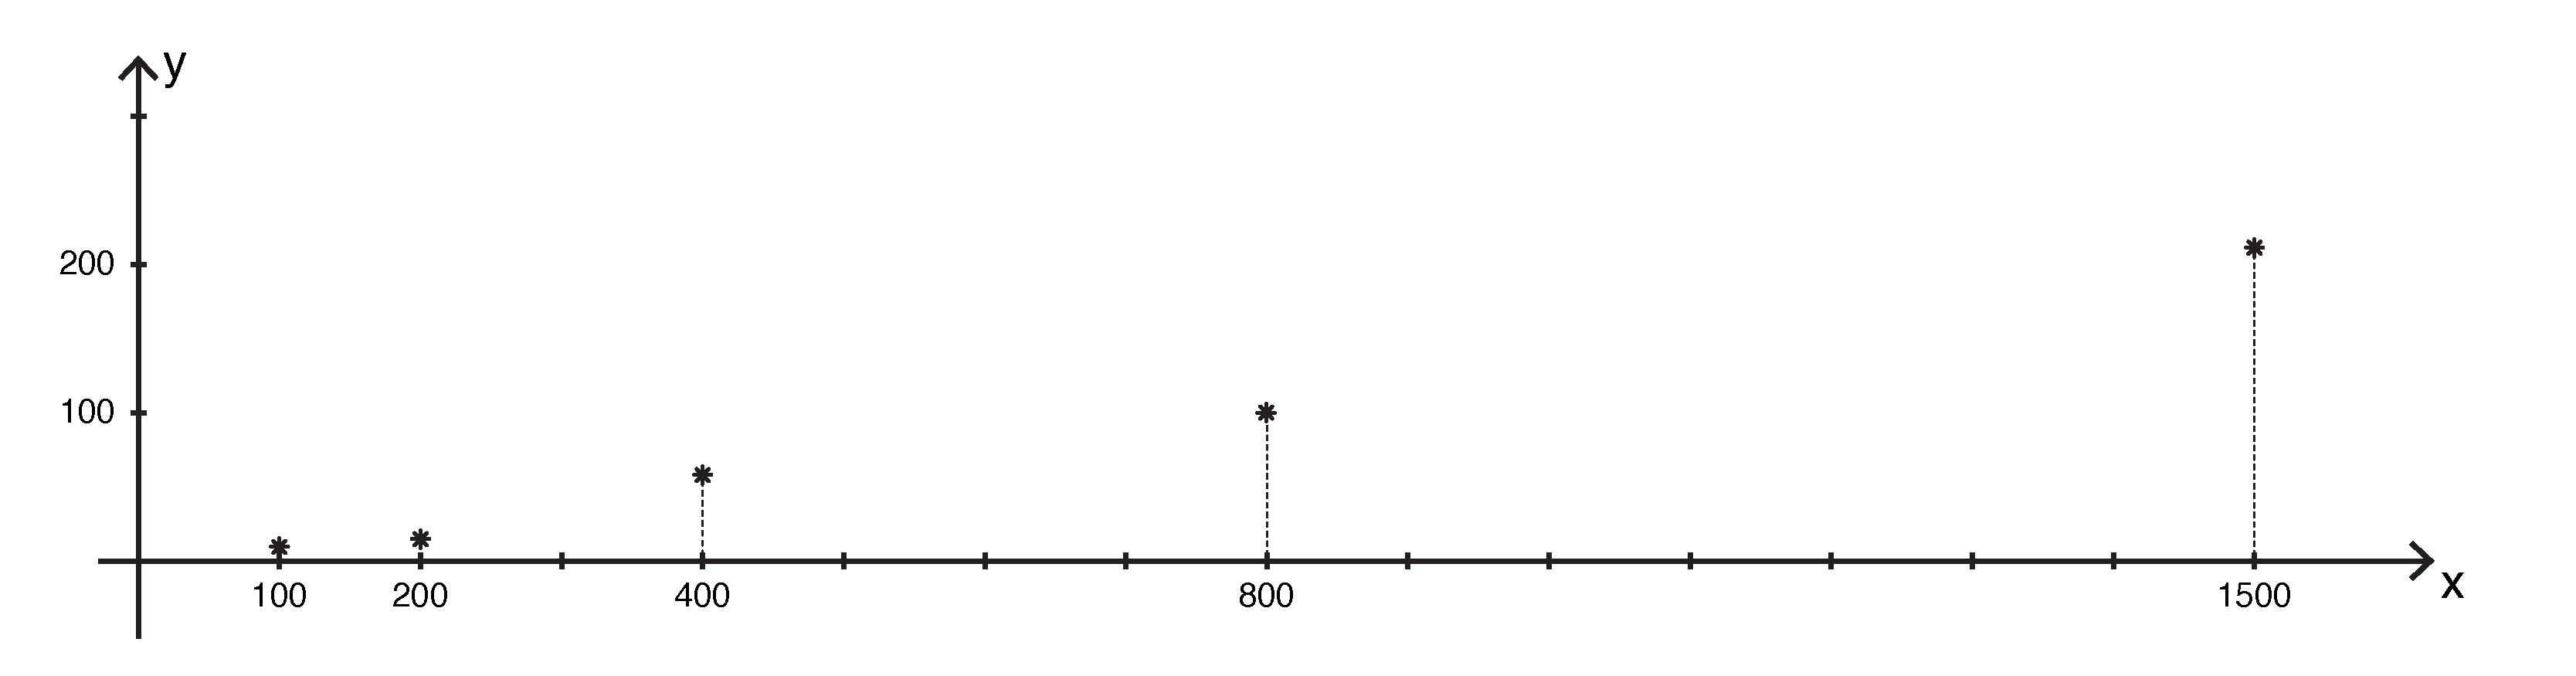
\includegraphics[width=1\textwidth]{images/b2p2-342-fig01}
            \end{figure}

            Taking the common logarithm of both sides of $y = k x^{r} $, we get the linear equation
                \[
                    \log y = \log k + r \log x
                \]
            in $ \log y $ and $ \log x $. Then setting 
            \[
                u = \log x, \quad v = \log y, \quad s = \log k
            \]
            we have 
        \end{hSolution}
    \end{exmp}
% =======================================================
\end{document}